\documentclass{article}
\usepackage[margin=1in]{geometry}
\usepackage{amsmath}
\usepackage{amssymb}
\usepackage{booktabs}
\usepackage{float}
\usepackage{graphicx}
\usepackage{hyperref}
\usepackage{pdfpages}
\usepackage{siunitx}
\usepackage{adjustbox}
\usepackage{cancel}
\usepackage{paracol}
\usepackage{placeins}

\usepackage{parskip}

\globalcounter{figure}
\counterwithin{equation}{section}

\title{Report}
\date{02 March 2026}
\author{Connor Emmons}

\begin{document}
\pagenumbering{gobble}
\maketitle
\vfill
\paragraph*{Notes}

\newpage
\pagenumbering{arabic}

\section{First Attempt at Fixing Hamiltonian - Final Velocity Free}

\subsection{Preliminary Implementation}

Changed the constraint that the full state had to be the same at the beginning and the end to only having to maintain $x$ and $y$ at the end. Then, the value to minimize is:

\begin{equation}
    \sqrt{\left(v_{xf} - v_{xi}\right)^2 + \left(v_{yf} - v_{yi}\right)^2}
\end{equation}

The solution ran very quickly ($\sim$0.1s) and the Hamiltonian was zero for every step; however, the orbit was incorrect. The solution is essetially the initial guess, as evidenced by the segmented nature of the orbit.

\begin{figure}[H]
    \centering
    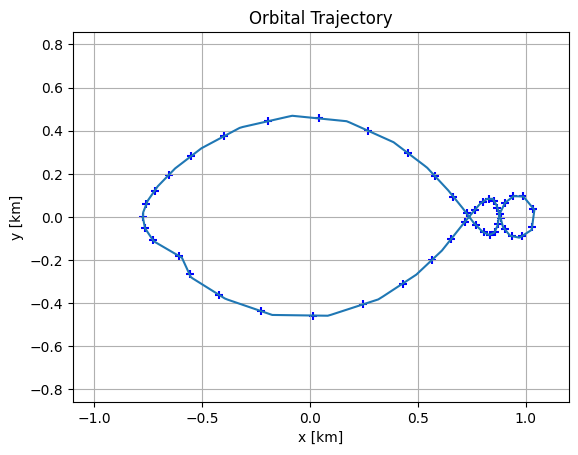
\includegraphics[width=\columnwidth]{orbit1.png}
    \caption{First orbit generated, note the segmented nature which reflects the manner that the initial guess is generated}
    \label{fig: orbit1}
\end{figure}

\begin{figure}[H]
    \centering
    
\includegraphics[width=\columnwidth]{jacobi1.png}
    \caption{The corresponding Jacobi constant, no good}
    \label{fig: jacobi1}
\end{figure}

Removing the bounds on time had no effect.

\subsection{Add Jacobi Constant to Cost}

Change the value to minimize to:

\begin{equation}
    \sqrt{\left(v_{xf} - v_{xi}\right)^2 + \left(v_{yf} - v_{yi}\right)^2} + W\int \left(C - C*\right)^2 dt
\end{equation}

Here, $C*$ is the targeted Jacobi constant and W is an adjustable weight. The first run with $W=1$ saw no change to the solution.

\begin{figure}[H]
    \centering
    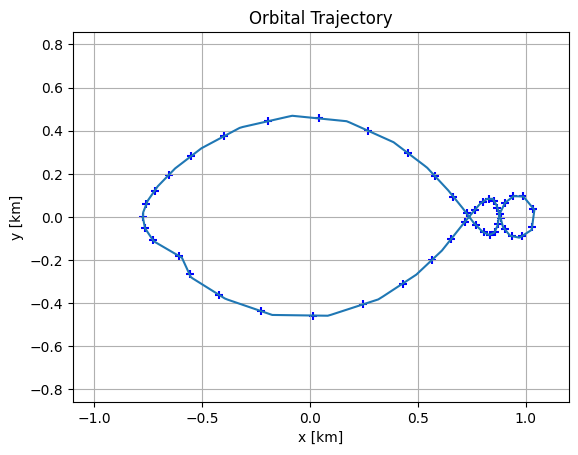
\includegraphics[width=\columnwidth]{orbit2.png}
    \caption{With W=1, no change}
    \label{fig: orbit2}
\end{figure}

Increasing $W$ to absurd numbers has no effect on the solution. In some way, this makes sense: the Jacobi constant is just a product of the dynamics of the system, which are already given. If YAPSS is ignoring the dynamics (which it is in the current solution), then adding in the Jacobi constant effectively does nothing.

\subsection{Add Control}

Now let YAPSS have control, specifically over the velocity. Now the goal is to minimize:

\begin{equation}
    \sqrt{\left(v_{xf} - v_{xi}\right)^2 + \left(v_{yf} - v_{yi}\right)^2} + \int W_c\left(C - C*\right)^2 + W_u\left(v_x^2 + v_y^2\right) dt
\end{equation}

This also resulted in no change to the solution. The orbit still mirrors the initial guess. Removing the Jacobi constant portion from the integral also had no effect. I am very confident that this implentation is garbage, and thus I have included a screenshot for future reference.

\begin{figure}[H]
    \centering
    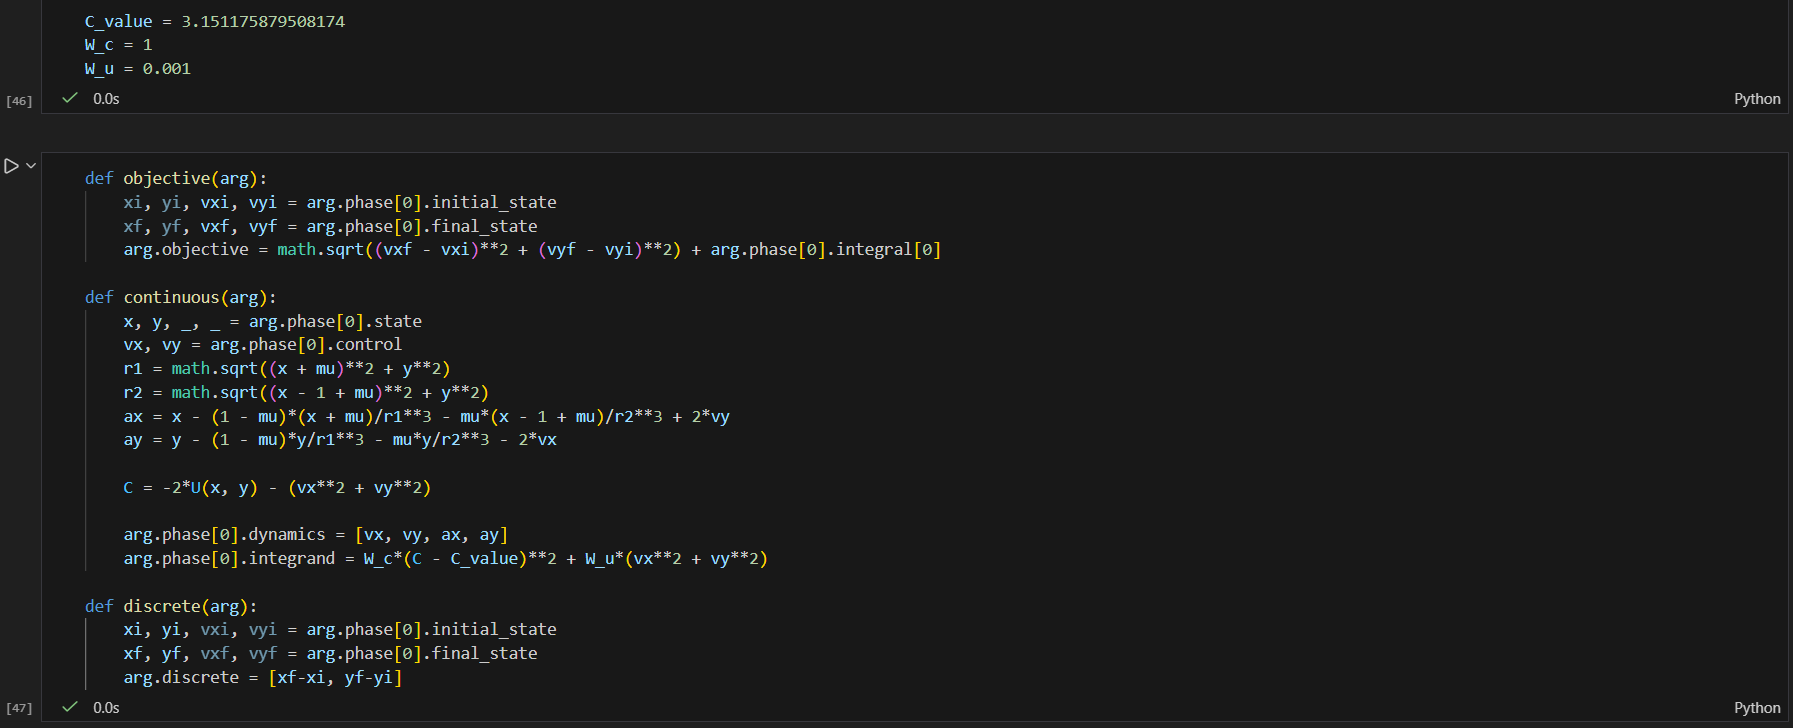
\includegraphics[width=\columnwidth]{code3.png}
    \caption{Code for control}
    \label{fig: code3}
\end{figure}

\subsection{Change Control to Acceleration}

Instead of having YAPSS control the velocity, have YAPSS be able to modify the acceleration by adding $ux$ and $uy$ to the corresponding accelerations. This also had absolutely no change on the solution, regardless of the weighting.

\section{New Idea - Velocity as Control}

Reduce the state to just the position and let YAPSS have full control over the velocity components. This was a dumb idea, and the orbit reflects this.

\begin{figure}[H]
    \centering
    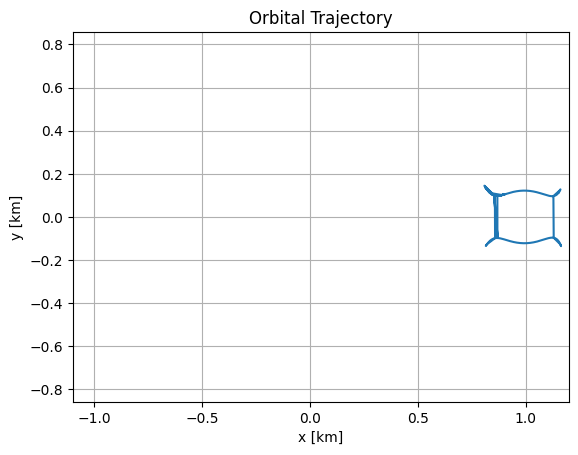
\includegraphics[width=\columnwidth]{orbit4.png}
    \caption{Result of a bad implementation}
    \label{fig: orbit4}
\end{figure}

\section{Good 2D Solution}

Instead, implement this properly as YAPSS being able to modify the velocity with the control. Additionally, remove the difference of the final velocities as part of the objective; This should be covered by the Jacobi constant and the control minimization. Thus, minimize:

\begin{equation}
    \int W_c\left(C - C*\right)^2 + W_u\left(v_x^2 + v_y^2\right) dt
\end{equation}

With both weights at 1, this generates a very good solution. The period error when compared to the paper is \num{2.59e-6} percent, or about 0.1 seconds. Even with no final constraint on either of the velocity components (though the x velocity is bounded to zero initially and finally to satisfy symmetry), the difference in y velocity is \num{2.11e-15}. The graphs look good and speak for themselves.

\begin{figure}[H]
    \centering
    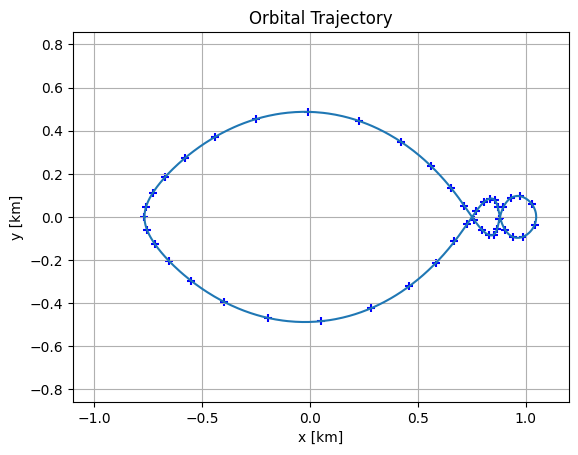
\includegraphics[width=\columnwidth]{good2dorbit.png}
    \caption{Good 2d orbit}
    \label{fig: good2dorbit}
\end{figure}

\begin{figure}[H]
    \centering
    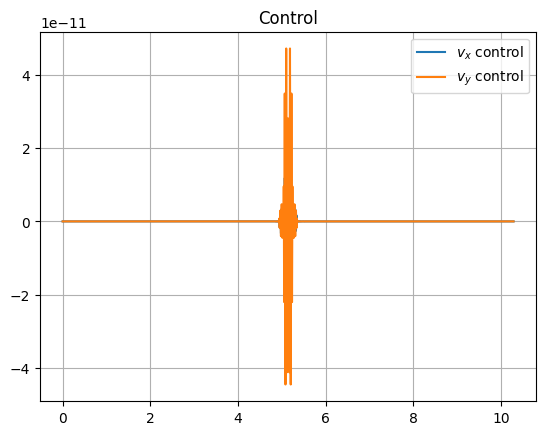
\includegraphics[width=\columnwidth]{good2dcontrol.png}
    \caption{Control for good orbit}
    \label{fig: good2dcontrol}
\end{figure}

\begin{figure}[H]
    \centering
    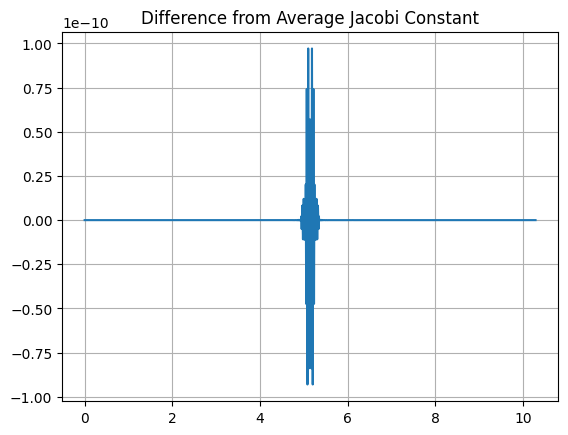
\includegraphics[width=\columnwidth]{good2djacobi.png}
    \caption{Jacobi difference for good orbit}
    \label{fig: good2djacobi}
\end{figure}

\begin{figure}[H]
    \centering
    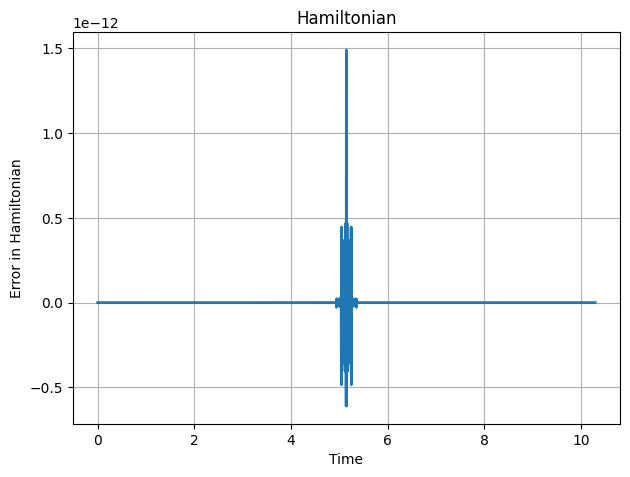
\includegraphics[width=\columnwidth]{good2dhamiltonian.png}
    \caption{Hamiltonian for good orbit}
    \label{fig: good2dhamiltonian}
\end{figure}

\section{Better 2D Solution}

I realized that I was defining my initial guess for the velocities incorrectly, and after fixing that, the solutions found were on the order of \num{1e-23} time units long. Without a final cost, YAPSS would apply a large amount of control and ignore the Jacobi constant to just keep the spacecraft in place, which was the minimal value on account of the short time step. To solve this, I added the final Jacobi constant difference as a part of the cost. Thus, minimize:

\begin{equation}
    W_{cf}\left(C_f - C*_f\right)^2 + \int W_c\left(C - C*\right)^2 + W_u\left(v_x^2 + v_y^2\right) dt
\end{equation}

This works very well. Period error is roughly 160 seconds (0.004 percent). The Jacobi is on the order of \num{1e-10}, the Hamiltonian is on the order of \num{1e-12}, and the controls demanded are on the order of \num{1e-11}. Below is a figure of the plot.

\begin{figure}[H]
    \centering
    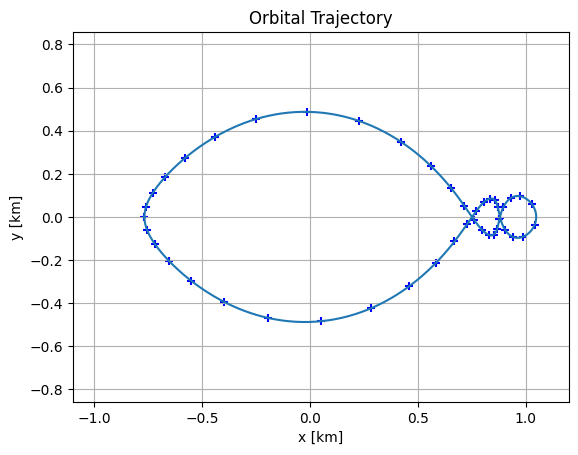
\includegraphics[width=\columnwidth]{better2dorbit.png}
    \caption{Fixed initial guess and cost functional}
    \label{fig: better2dorbit}
\end{figure}

\section{Extending to 3D}

This approach was extended to the 3D model. After adjusting the dynamics and the Jacobi constant equation accordingly, the results roughly match. Note that the final solution for the 2D orbit is used as the initial guess for the 3D orbit. Additionally, while the 2D model takes about 7 seconds to find a solution, the 3D model takes about 3 minutes. The period error dropped to 20 seconds, or 0.0005 percent.

\begin{figure}[H]
    \centering
    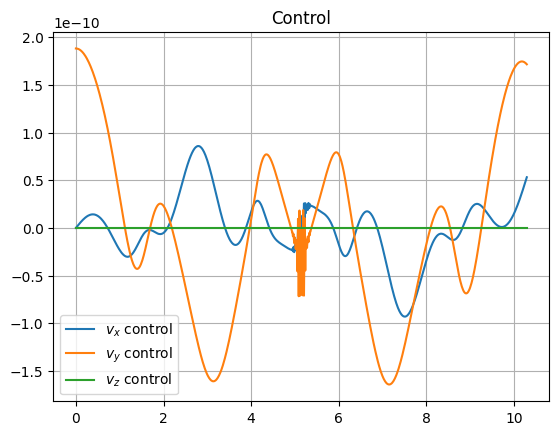
\includegraphics[width=\columnwidth]{3dcontrol.png}
    \caption{Control for 3D orbit}
    \label{fig: 3dcontrol}
\end{figure}

\begin{figure}[H]
    \centering
    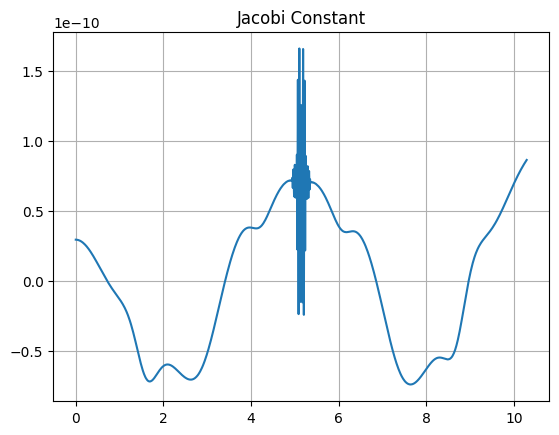
\includegraphics[width=\columnwidth]{3djacobi.png}
    \caption{Jacobi for 3D orbit}
    \label{fig: 3djacobi}
\end{figure}

\begin{figure}[H]
    \centering
    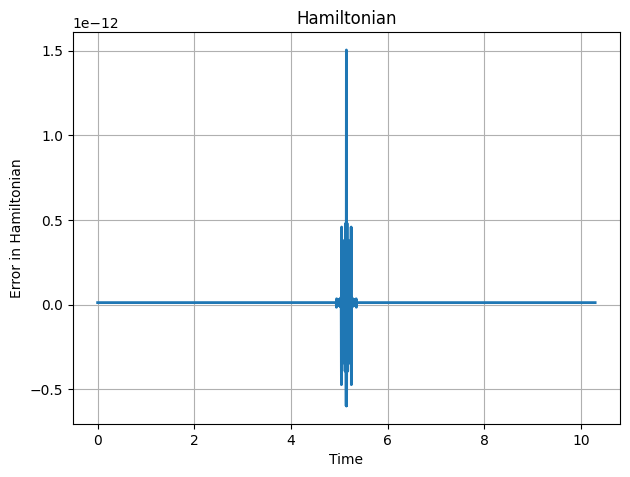
\includegraphics[width=\columnwidth]{3dhamil.png}
    \caption{Hamiltonian for 3D orbit}
    \label{fig: 3dhamil}
\end{figure}

\end{document}